\def\mytitle{Coursework Report}
\def\mykeywords{Fill, These, In, So, google, can, find, your, report}
\def\myauthor{Samuel Cattanach}
\def\contact{40276600}
\def\mymodule{SET09122 Artificial Intelligence}
\documentclass[12pt, a4paper]{article}
\usepackage[a4paper,outer=2cm,inner=2cm,top=2cm,bottom=2cm]{geometry}
\onecolumn
\usepackage{graphicx}
\graphicspath{{./images/}}
\usepackage[colorlinks,linkcolor={black},citecolor={blue!80!black},urlcolor={blue!80!black}]{hyperref}
\usepackage[parfill]{parskip}
\IfFileExists{uarial.sty}
{
    \usepackage[english]{babel}
    \usepackage[T1]{fontenc}
    \usepackage{uarial}
    \renewcommand{\familydefault}{\sfdefault}
}{
    \GenericError{}{Couldn't find Arial font}{ you may need to install 'nonfree' fonts on your system}{}
    \usepackage{lmodern}
    \renewcommand*\familydefault{\sfdefault}
}
\usepackage{watermark}
\usepackage{xcolor}
\usepackage{listings}
\usepackage{float}
\usepackage{titlesec}
\usepackage{amsmath}
\usepackage{algorithm2e}
\titlespacing{\subsection}{0pt}{\parskip}{-3pt}
\titlespacing{\subsubsection}{0pt}{\parskip}{-\parskip}
\titlespacing{\paragraph}{0pt}{\parskip}{\parskip}
\newcommand{\figuremacro}[5]{
    \begin{figure}[#1]
        \centering
        \includegraphics[width=#5\columnwidth]{#2}
        \caption[#3]{\textbf{#3}#4}
        \label{fig:#2}
    \end{figure}
}
\lstset{
	escapeinside={/*@}{@*/}, language=C++,
	basicstyle=\fontsize{8.5}{12}\selectfont,
	numbers=left,numbersep=2pt,xleftmargin=2pt,frame=tb,
    columns=fullflexible,showstringspaces=false,tabsize=4,
    keepspaces=true,showtabs=false,showspaces=false,
    backgroundcolor=\color{white}, morekeywords={inline,public,
    class,private,protected,struct},captionpos=t,lineskip=-0.4em,
	aboveskip=10pt, extendedchars=true, breaklines=true,
	prebreak = \raisebox{0ex}[0ex][0ex]{\ensuremath{\hookleftarrow}},
	keywordstyle=\color[rgb]{0,0,1},
	commentstyle=\color[rgb]{0.133,0.545,0.133},
	stringstyle=\color[rgb]{0.627,0.126,0.941}
}
\thiswatermark{\centering \put(330.5,-38.0){
\includegraphics[scale=0.8]{logo}} }
\title{\mytitle}
\author{\myauthor\hspace{1em}\\\contact\\Edinburgh Napier University\hspace{0.5em}-\hspace{0.5em}\mymodule}
\date{}
\hypersetup{pdfauthor=\myauthor,pdftitle=\mytitle,pdfkeywords=\mykeywords}
\sloppy

% #######################################
% ########### START FROM HERE ###########
% #######################################
\begin{document}
    \maketitle

% \section{Introduction}

    % (12 Marks – maximum two pages) description of Dijkstra's algorithm with enough detail for someone to be able to implement it to solve the cave problem. 
    % diagrams which help understand the text, directly relevant to the problem. 
    % evaluation of the algorithm explaining the situations where it is more or less useful.
\section{Dijkstra's Shortest Path First Algorithm}
    %description
    First published in 1959 by Edsger Dijkstra, Dijkstra's shortest path first algorithm is the basis of many path-finding artificial intelligence and has been expanded upon by several algorithms such as A*. One of the main applications of Dijkstra's algorithm is finding the quickest routes between physical locations using paths such as roads. The algorithm is implemented to be able to find the optimal route, if a route exists, in any scenario. the information required to find a path is a specific starting node, an end node, and either the coordinates of all nodes or the distances between each node. Starting at the specified node, Dijkstra's algorithm will first use the connectivity matrix in order to go through all of the other nodes in order to find which ones can be visited from the starting node. For each neighbouring node that can be visited the distance of each is calculated. the neighbor which has the shortest distance traveled so far is selected as the next node regardless of whether it is closer to the specified end node or not. Two lists are maintained throughout the calculation of the shortest path. The first list is a priority queue consisting of nodes which have not been fully investigated yet which is sorted by the shortest distance first. The second list contains all of the nodes which have been fully investigated and will not be looked at again. Firstly, the traversable neighbouring nodes from the start point will be added to the priority queue and will have their traveled distances and parent nodes recorded along with their coordinates. The starting node, once all traversable neighbouring nodes are added to the priority queue, will be added to the second list of investigated nodes. The algorithm then continues through the nodes, calculating the shortest routes first, until the end node is reached. Once the goal has been reached, the final path traversed is established by following the parent of each node until a path from the first node to the end node has been established. Through proper implementation of Dijkstra's algorithm the optimal path from start to finish will always be found.
    
    \begin{figure}[!htb]
    \centering
    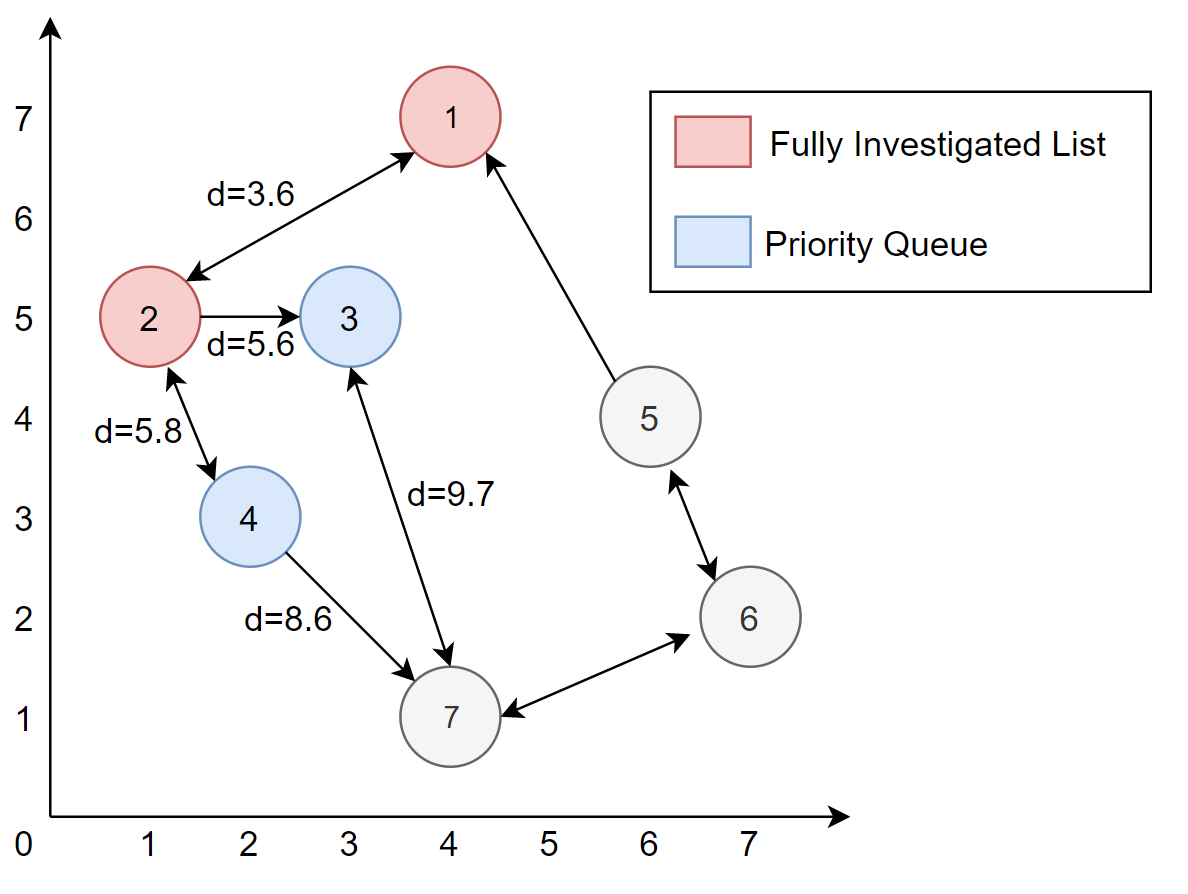
\includegraphics[height=8cm]{d.png}
    \caption{Dijkstra's algorithm} \label{fig1}
    \end{figure}
    
    In regards to the cave problem described previously, Dijkstra's algorithm can be implemented in order to find the optimal route of any series of caves, and will also be able to identify if no route  to the end cave is available. As the Euclidean distance can be calculated using each caves coordinates and a connectivity matrix of all of the caves is supplied, Dijkstra's algorithm will be able to start at cave one and work through every traversable neighbouring node until the last cave is reached.
    % evaluation
    Dijkstra's shortest path first algorithm was first implemented on the ARMAC computer which had only 15 kilobytes of memory, because of this small amount of memory, there were limitations in how advanced Dijkstra's algorithm could be. The most major limitation in comparison to some of its successors was that it did not take into account any heuristic value for the nodes. 
\newpage
Since only the distance travelled so far is taken into consideration and not the distance from the end node, the algorithm may first calculate nodes leading away from the end node before going back towards it.
    % where it's most usefull
    Dijkstra's algorithm is usually implemented in uninformed environments, where a heuristic value can not be assigned to nodes, and the distance or cost between nodes may not be previously known. In this situation, with the absence of knowledge of the complete graph, Dijkstra's algorithm performs the same as with the A* algorithm as h(n) is 0 for every node and calculations can only be made based on g(n).
    % where it's least usefull
    Unlike with greedy best-first-search algorithms, because Dijkstra's algorithm does not move towards the end goal specifically but in an outwards motion from the start node, it can be very slow in comparison. As a result of this slow computational speed, the algorithm is inferior to others when used as an AI path-finding algorithm in some video games. Where there may not be many obstacles in the way of the start and end node, or the connectivity between nodes is high, the algorithm will waste time computing nodes which are farther away from its goal, shown in figure 2.

    \begin{figure}[!htb]
    \centering
    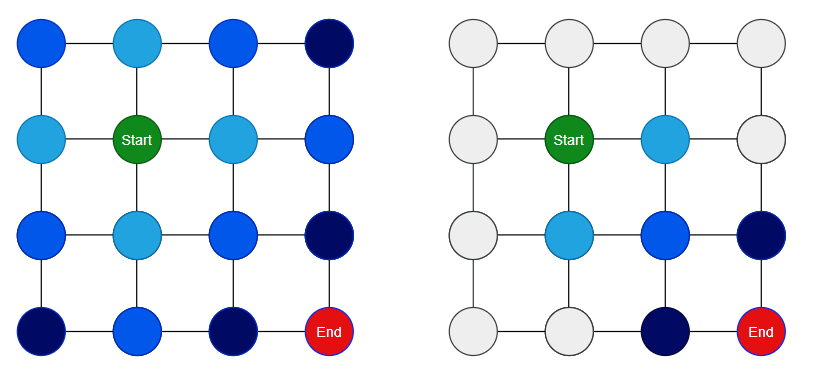
\includegraphics[height=7cm]{DvsA.png}
    \caption{Dijkstra's algorithm (left) compared to A* (right)} \label{fig2}
    \end{figure}


    % (13 Marks – maximum one page) Identify (don’t describe) a good algorithm to use for solving the problem and explain why it is good for this problem. 
\section{The A* Path-Finding Algorithm}
The informed best-first A* algorithm, first published in 1968 is widely considered the "most popular choice for path-finding, because it is fairly flexible and can be used in a wide range of contexts" (Patel, 2009)\cite{Patel}.  Given the limitations of Dijkstra's algorithm, one of its successors, the A* search algorithm allows for an optimal route to be discovered much faster in informed environments.  A* would be a more suitable choice of algorithm for the given problem of navigating a system of connected caves because it takes into consideration not only the distance travelled, but a heuristic value as well. This heuristic value may be the Euclidean distance or the Manhattan distance for example. By calculating the Euclidean distance of each node (h(n)) and the exact distance travelled so far (g(n)), using the below formula (Fig 3) to determine which node to explore first provides an optimal solution at a much faster rate. If an ineffective heuristic value is given for each node the computational time will increase, although still faster or just as fast as Dijkstra's algorithm, but an optimal route will always be found.
    
    \begin{figure}[!htb]
    \centering
    \fontsize{15pt}{15pt}\selectfont
    \begin{verbatim}
                        f(n) = g(n) + h(n)
    \end{verbatim}
    \caption{ A* shortest-first algorithm} \label{fig3}
    \end{figure}
    
    % If the problem were to change so that the cost of taking a particular tunnel in a particular direction is given in the file – no-longer related to distance travelled, explain how this might affect your choice of algorithm and identify any problem that might occur in this situations.
    In a situation where instead of using the Euclidean distance as the distance travelled, each tunnel in a particular direction had a specified cost, the A* algorithm would not be the most suitable choice in finding an optimal path. In this scenario, the only given information to use when deciding which node to explore first is g(n), the exact distance travelled so far. No heuristic value can be assigned to each node and therefor A* should not be used as it is an informed best-first search.
    Instead of using A* in this situation, Dijkstra's algorithm is the more suited implementation as it only requires a g(n) value and is preferable in uninformed environments.
    
    
    
    
% \section{Conclusion}

%\bibliographystyle{splncs04}
%\bibliography{mybibliography}
%
\begin{thebibliography}{8}
\bibitem{Patel}
Patel, A. (2009). Introduction to A*. Retrieved from \url{http://theory.stanford.edu/~amitp/GameProgramming/AStarComparison.html}.


\end{thebibliography}		
\end{document}


